229. \begin{figure}[ht!]
\center{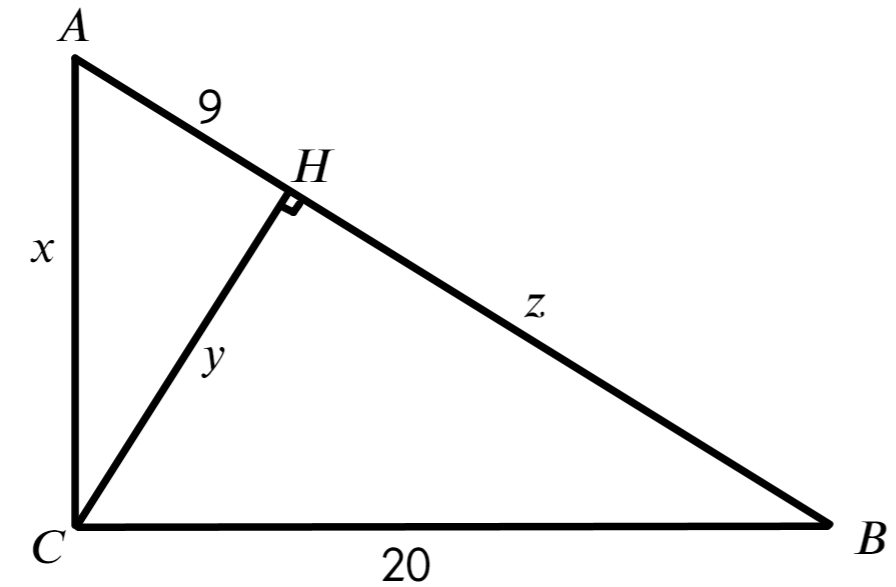
\includegraphics[scale=0.35]{g8-229.png}}
\end{figure}\\
Пусть $AC=x,\ CH=y,\ HB=z.$ Тогда из теорем Пифагора для прямоугольных треугольников $ACH,\ BCH$ и $ABC$ имеем систему уравнений $\begin{cases} y^2+81=x^2,\\ y^2+z^2=400,\\ x^2+400=(z+9)^2.\end{cases}$ Сложив все левые части и все правые, получим соотношение $2y^2+z^2+x^2+481=x^2+481+z^2+18z,\ 2y^2=18z,\ y^2=9z.$ Тогда $9z+z^2=400,\ z^2+9z-400=0,\ (z-16)(z+25)=0,\ z=16$см. Значит, $y^2=9\cdot16,\ y=3\cdot4=12$см. Тогда $S_{\Delta ABC}=\cfrac{1}{2}\cdot12\cdot(9+16)=150\text{ см}^2.$\\
